\documentclass[12pt,a4paper]{article}
\usepackage[latin1]{inputenc}
\usepackage[spanish,activecute]{babel}
\usepackage{amsmath}
\usepackage{amsfonts}
\usepackage{amssymb}
\usepackage{graphicx}
\usepackage[hidelinks]{hyperref}
\usepackage[left=1.5cm,right=1.5cm,top=1.5cm,bottom=1.5cm]{geometry}
\author{MEJORADA LOPEZ IVAN}
\title{OPERACION DE LOS CIRCUITOS DE ACTIVACION CON TIRISTORES EN CONVERTIDORES CA-CD Y CA-CA}
\maketitle

\includegraphics[width=\textwidth]{UPZMG_Prueba_1b.png} 
\newpage
\section{Que son los circuitos de activacion}
hay distintos tipos de circuitos de activacuon, los mas comunes son con diodos triacs, leds, etc. Estos tambien pueden usarse con los tristores en algunos convertidores de CA-CD y CA-CA, como podemos observar en los siguientes diagramas 
\\
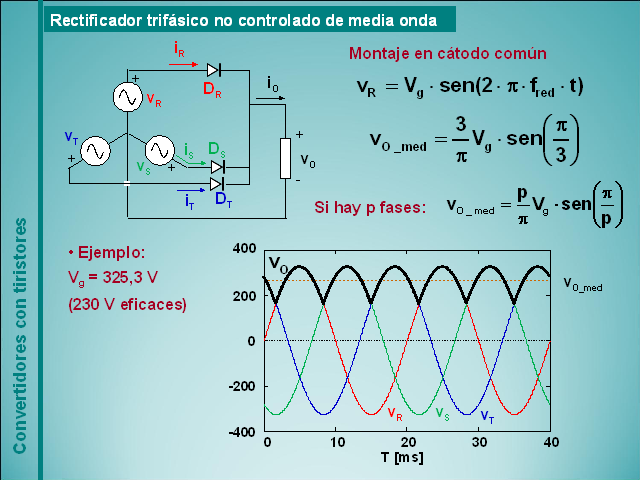
\includegraphics[width=\textwidth]{img2.png} 
\newpage
\section{Que son los tristores }
El tiristor es un semiconductor de potencia que se utiliza como interruptor, ya sea para conducir o interrumpir la corriente electrica, a este componente se le conoce como de potencia por que se utilizan para manejar grandes cantidades de corriente y voltaje, a comparacion de los otros semiconductores que manejan cantidades relativamente bajas.\\Cuando se habla de tiristores comunmente se cataloga al tiristor como un SRC (silicon controlled rectifier), pero esto no es del todo correcto ya que este tipo es el mas popular y conocido pero no es el unico que existe

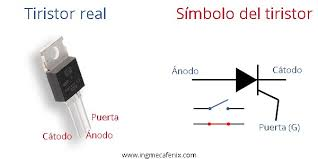
\includegraphics[width=\textwidth]{descarga.jpeg} 

\section{CONVERTIDORES CON TRISTORES}
Convertidores con tiristores Hasta los a\~{n}os 70, la mayor parte de la electr\`{o}nica de potencia se basaba en el uso de tiristores (especialmente SCRs) como interruptores controlados Con SCRs se dise\~naban convertidores CC/CC, CC/CA, CA/CC y CA/CA En la actualidad, en la mayor\'ia de las aplicaciones de electr\'onica de potencia los interruptores controlados son MOSFETs o IGBTs (a potencias muy altas se siguen utilizando SCRs y GTOs) Nosotros vamos a estudiar los siguientes convertidores basados en tiristores:Convertidores CA/CC: Rectificadores trifásicos controlados (con SCRs) Rectificadores trif\'asicos semicontrolados (con SCRs y diodos) Convertidores CA/CA: Controladores de fase monof\'asicos (con triacs)
\newpage
\section{Convertidores con tiristores Rectificador trif\'asico no controlado de media onda}
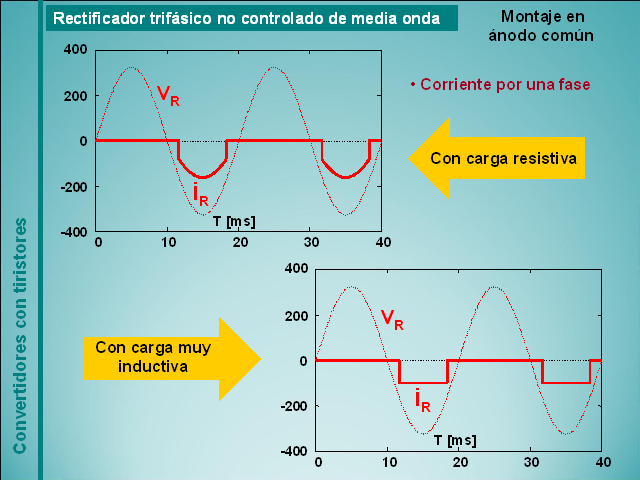
\includegraphics[width=10cm]{img5.png} 
\section{Convertidores con tiristores Rectificador trif\'asico no controlado de onda completa}
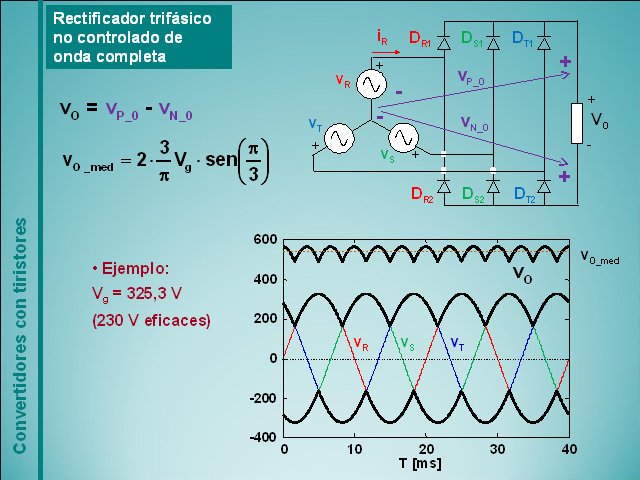
\includegraphics[width=10cm]{img6.png}
\newpage
\section{CONVERTIDORES MODERNOS SIN TRISTORES}
Tambien existen convertidores modernos el cual vienen sin tristores, por la tecnologia que puede llegar a tener, en las siguintes imagenes les mostraremos cuales son los vonvertidores modernos 
\subsection{MODERNOS}
Convertidores con tiristores Con el control adecuado de los interruptores se puede conseguir controlar la corriente por las entradas (que puede ser senoidal en fase con la tensi\'on) y la tensi\'on de salida Con interuptores bidireccionales en corriente y tensi\'on se puede conseguir que el rectificador funcione como inversor suministrando corriente senoidal en fase con la tensi\'on de entrada Su estudio no se puede abordar en esta asignatura Rectificadores trif\'asicos modernos (sin tiristores)\\
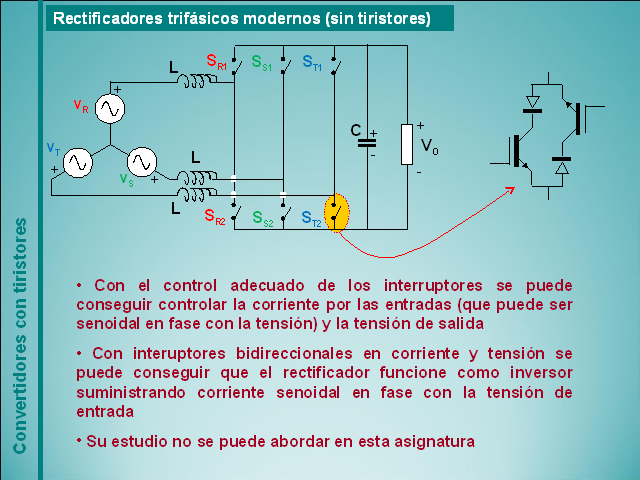
\includegraphics[width=10cm]{img27.png} 
\subsection{MODERNOS}
Convertidores con tiristores El convertidor Back to Back Rectificadores trif\'asicos modernos (sin tiristores)\\
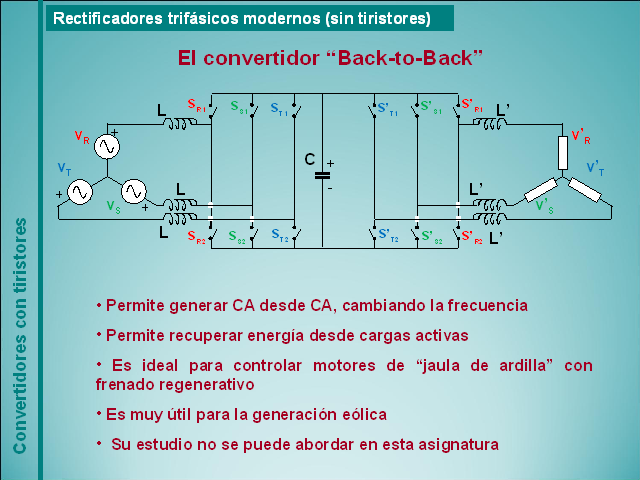
\includegraphics[width=8.8cm]{img28.png} 
\section{convertidores CA-CA}
Convertidores con tiristores Reciben el nombre de controladores de fase Convertidores CA /CA monof\'asicos sin cambio de frecuencia Es un circuito muy utilizado (control de intensidad luminosa, control de velocidad de motores de colector, control continuo de calefacci\'on el\'ectrica, etc.) Cuando la tensi\'on en el condensador C1 alcanza la tensi\'on de disparo del DIAC DI1 (t\'ipicamente 30 V), se dispara el TRIAC TR1 y, por tanto, se aplica tensi\'on a la carga El instante en el que se dispara el DIAC depende de la resistencia variable Rv. Controlando su valor se controla el \'angulo de desfase a y, por tanto, la potencia aplicada a la carga\\
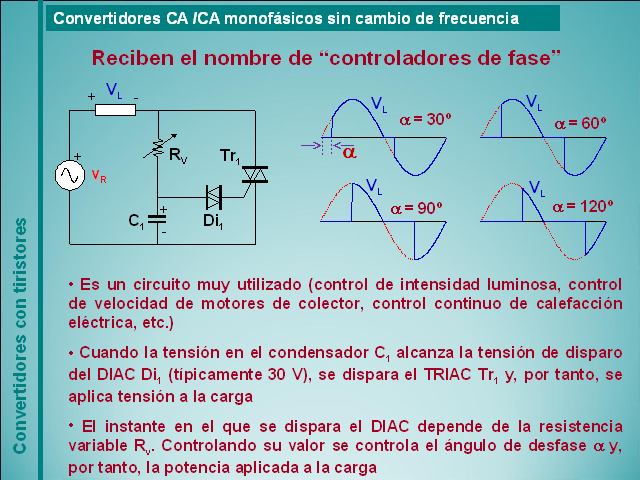
\includegraphics[width=20cm]{img29.png} 
\newpage
\section{BIBLIOGRAFIAS}
\url{https://www.ingmecafenix.com/electronica/que-es-un-tiristor-y-como-funciona/}
\\
\url{https://www.monografias.com/trabajos105/convertidores-ca-cc-y-ca-ca-tiristores/convertidores-ca-cc-y-ca-ca-tiristores.shtml}
\\
\url{http://ccpot.galeon.com/enlaces1737112.html}
\\
\url{https://ingenieriaelectronica.org/circuitos-de-activacion-para-diodos-laser/}






\end{document}
